\documentclass{scrartcl}
\usepackage[utf8]{inputenc}
\usepackage{hyperref}
\usepackage{url}
\usepackage{natbib}
\usepackage{graphicx}
\usepackage{minted}
\usepackage{csquotes}
\usepackage{pdflscape}

\newcommand{\emailaddr}[1]{\href{mailto:#1}{\texttt{#1}}}

\title{\LARGE Understanding the behaviour of BDI agents through incremental sifting of execution traces }

\author{ Riccardo Battistini 0001034968 \\ \emailaddr{riccardo.battistini2@studio.unibo.it} }

\date{June 2025}

\begin{document}

\maketitle

\begin{abstract}
    The goal of this project is to develop a system for explaining, debugging, and validating the behavior of BDI (Belief-Desire-Intention) agents through the reimplementation of a multi-level explainability framework, using a set of declarative sifting patterns. The system aims to bridge the gap between technical implementation details and human-understandable explanations of agent behavior by providing a DSL that allows to extract higher-level narratives out of raw execution traces.
\end{abstract}

\section{Requirements}

\begin{itemize}
\item Develop a logging module integrated with a BDI agent platform to capture the execution traces of agents' behavior at the implementation level.
\item Enable the definition of domain-specific patterns with declarative rules.
\item Provide a clear separation between pattern definition and pattern matching logic.
\item Support incremental matching for online processing requirements.
\end{itemize}

\subsection{Expected Outcomes}

\begin{itemize}
\item A monitoring and validation system for BDI agent behavior.
\item Generation of narratives that make agent decisions and behaviors comprehensible to different stakeholders.
\item Improved debugging and development workflows for multi-agent systems.
\end{itemize}

\subsection{Scenarios}

\subsubsection{Developer Debugging Session}

\begin{itemize}
    \item Who: software developers working on BDI agent systems.
    \item How: developers access implementation-level traces through the console, the file browser or a dashboard.
    \item Why: to identify and resolve bugs faster.
\end{itemize}

\subsubsection{System Designer Review}

\begin{itemize}
    \item Who: system architects and designers.
    \item How: designers examine domain-level narratives to validate that agent behavior aligns with intended BDI model specifications.
    \item Why: to ensure the implemented system correctly reflects the designed agent architecture and decision-making processes.
\end{itemize}

\subsubsection{Anomaly Detection}

\begin{itemize}
    \item Who: system administrators.
    \item How: continuous monitoring of agent behavior with automatic alerts when predefined patterns indicate potential issues.
    \item Why: to proactively identify and address system anomalies.
\end{itemize}

\section{Requirements Analysis}
\subsection{Implicit Requirements}

\begin{itemize}
    \item Performance: logging should not significantly impact agent execution performance.
    \item Scalability: the pattern-matching engine should be efficient and capable of handling a large volume of log events (thousands) with a significant number of patterns (tens). In addition it should be able to handle multiple concurrent agents.
    \item Structure: structured logging should be used to enable efficient pattern matching and data extraction from log entries without needing to implement custom parsers.
\end{itemize}

\subsection{Implicit Hypotheses}

\begin{itemize}
    \item Pattern expressiveness: the Winnow DSL and its Kotlin reimplementation are sufficiently expressive to capture the semantic mappings required for meaningful transitions of abstraction levels.
    \item Domain generalization: patterns developed for one domain can be adapted or serve as templates for other domains.
\end{itemize}

\subsection{Non-functional requirements}

\begin{itemize}
    \item Extensibility: the definition of sifting patterns should accommodate new domains and use cases without requiring modifications of the system's architecture.
    \item Compatibility: the system must integrate with existing JaKtA applications without requiring significant modifications.
\end{itemize}

\section{Design}

The JaKtA BDI interpreter \cite{DBLP:conf/eumas/BaiardiBCP23} has been chosen as a base for implementing the project.

The project is organized in three modules:

- \verb|jakta-bdi|: the logging module is part of the BDI engine. Most of the code contributed is under the \verb|it.unibo.jakta.agents.bdi.engine.logging| and the \\ \verb|it.unibo.jakta.agents.bdi.engine.executionstrategies.feedback| packages.

- \verb|jakta-playground|: includes the domestic robot application and an example set of sifting patterns to build a narrative that explains the behavior of the agents.

- \verb|jakta-narrative-generation|: includes both the engine to perform the matching of the patterns and an internal DSL in Kotlin to declare them.

\subsection{Logs as narratives}

The explainability framework outlined in \cite{DBLP:journals/aamas/YanBHR25} has been used as a reference for this project. The framework has two main components:

\begin{itemize}
    \item the logging component, which is analogous to the logging module part of \verb|jakta-bdi|;
    \item the explanation component, which is partially implemented in the \\ \verb|jakta-narrative-generation| module.
\end{itemize}

The explanation component generates explanations at three levels of abstraction:

\begin{itemize}
    \item the implementation level. It provides a narrative suitable for developers. It’s very close to the raw logs produced by the system execution. It follows the operational semantics of the programming language used to code the agent and of the platform on which it is run. It details the inner workings of the agent;
    \item the design level. It provides a narrative suitable for designers. It’s based on the BDI
abstraction. It provides a first person account of the agent behavior, reporting events
related to its lifecycle;
    \item the domain level. It provides a narrative suitable for end users and domain experts. It
provides explanations in terms of the system’s requirements and of its domain, in a way
similar to the user stories. It’s application-specific.
\end{itemize}

Each level is defined on top of the previous level.

Winnow is a domain-specific language for incremental story sifting built on top of Datalog and
Datascript \cite{DBLP:conf/aiide/KreminskiDM21}.
%
It is conceived to extract compelling sequences of events from a corpus of narrative material. 

Embracing the view of logs as narratives to explain and understand, as
proposed in \cite{DBLP:journals/aamas/YanBHR25}, Winnow can be used to write declarative rules that map sequences of events to higher level patterns defined at an increased level of abstraction.
%
The sifting patterns can be used to generate explanations and to detect potential rule violations
as they unfold during the execution of a multi-agent system, increasing the transparency of
the system and allowing to anticipate potential issues.

The project uses the logging module to create execution traces of log events defined at the implementation level. 
%
The narrative-generation module allows to match a set of given sifting patterns to map those log events to a new sequence of events defined at the domain-level.

\subsection{The logging system}

The logging system is based on the interfaces \verb|LogEventContext| and \verb|LogEvent|.
%
The first interface acts as a wrapper of \verb|LogEvent|s and provides information used to univocally identify each event with the id of the Mas execution and the id of the agent, if relevant for the event.
%
\verb|LogEvent| is the base interface from which all other log events extend. In figure \ref{fig:jakta-log-event} the base hierarchy is shown. There are three main kinds of events:

\begin{itemize}
    \item \verb|ExecutionFeedback| references events relative to the result of the execution of the sense-reason-act cycle. This includes whether relevant or applicable plans are not found during the deliberation or if the execution of an action fails in the action phase. In figure \ref{fig:execution-feedback} all the feedback events provided by the BDI engine are shown. By extending the interface, the user can record new kind of feedback as a result of the execution of custom actions.
    \item \verb|EnvironmentEvent| references the effects that are applied to the environment after the execution of the deliberation cycle of an agent. This includes for example receiving, sending or broadcasting messages. In figure \ref{fig:environment-change} all the log events relative to the environment provided by the BDI engine are shown. By extending the interface, new kind of environmental conditions can be logged from user-provided environments.
    \item \verb|AgentEvent| references log events generated by each agent, relative to its internal mechanics and its data structures. For example, this includes events related to the selection, addition or removal of intentions, plans or events. In figures \ref{fig:jakta-log-event} and \ref{fig:agent-event} all the logged events are shown.
\end{itemize}

\begin{figure}
    \centering
    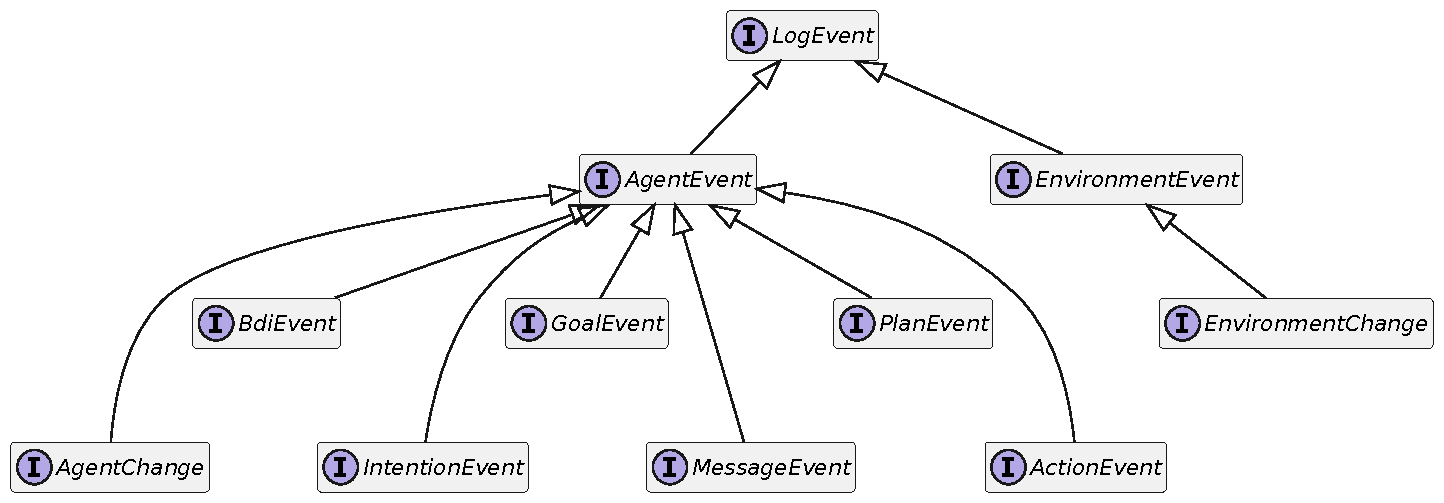
\includegraphics[width=\textwidth]{logEvent.pdf}
    \caption{LogEvent interface hierarchy.}
    \label{fig:jakta-log-event}
\end{figure}

\begin{figure}
    \centering
    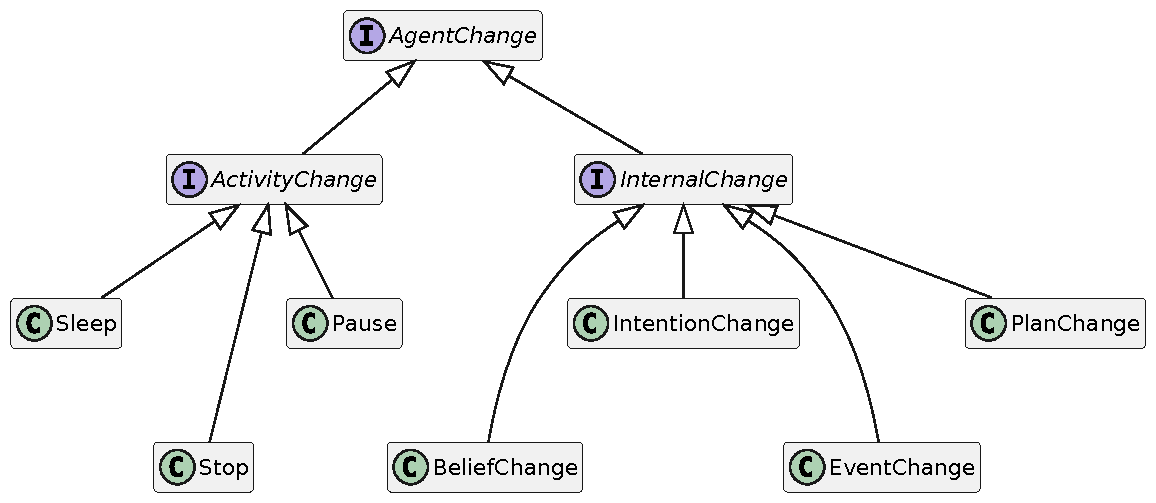
\includegraphics[width=\textwidth]{agentChange.pdf}
    \caption{AgentEvent interface hierarchy.}
    \label{fig:agent-event}
\end{figure}

\begin{figure}
    \centering
    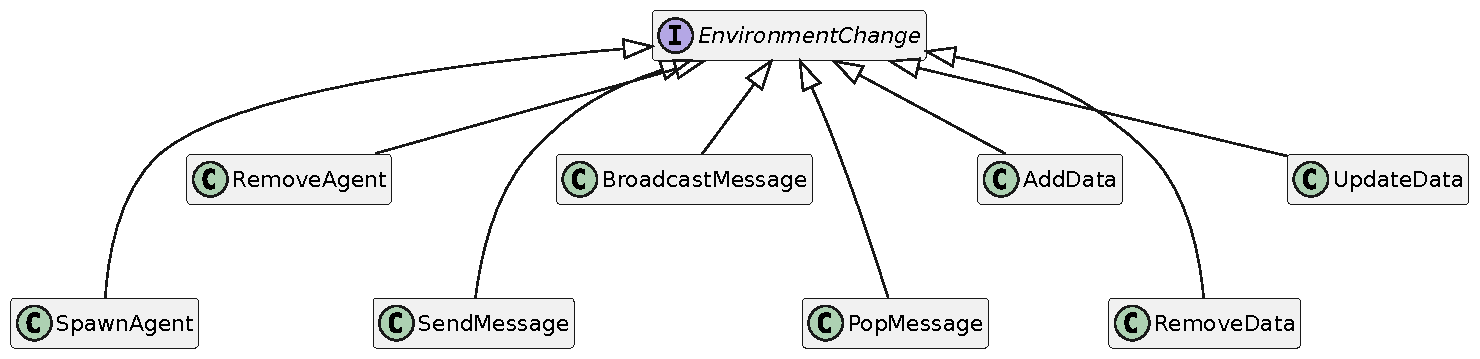
\includegraphics[width=\textwidth]{environmentChange.pdf}
    \caption{EnvironmentChange interface hierarchy.}
    \label{fig:environment-change}
\end{figure}

\begin{figure}
    \centering
    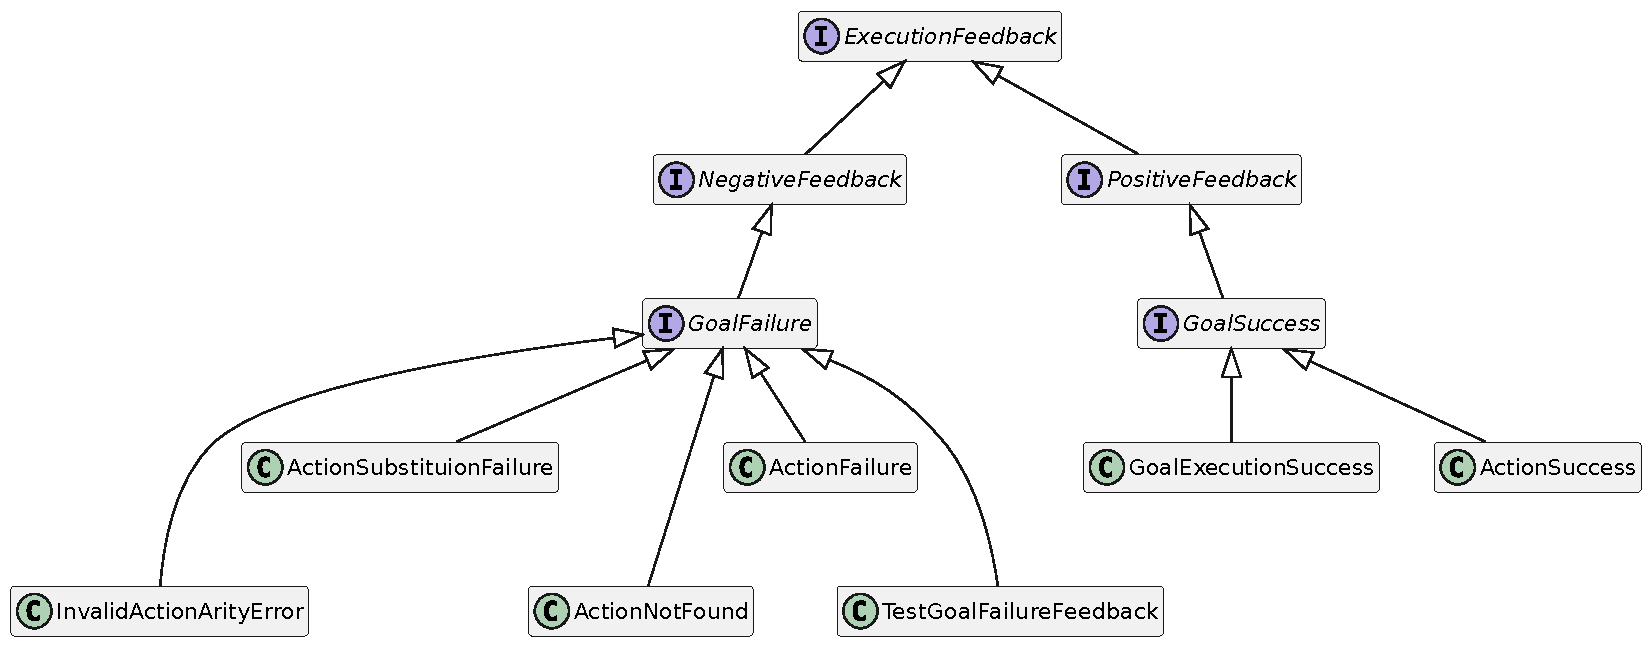
\includegraphics[width=\textwidth]{executionFeedback.pdf}
    \caption{ExecutionFeedback interface hierarchy.}
    \label{fig:execution-feedback}
\end{figure}

The \verb|JaktaLogger| interface provides the starting point from which the loggers are defined. It is implemented only by the \verb|MasLogger| and \verb|AgentLogger| interfaces and provides a set of functions to log strings or objects, according to the chosen log level.

If logging is enabled, during Mas initialization, a \verb|MasLogger| is created. Then each agent is equipped with an \verb|AgentLogger|. 
%
The former logger is used to log any \verb|EnvironmentEvent|,  namely any environmental effect, along with any custom user-provided environment event. The latter loggers are used to log any kind of \verb|AgentEvent|.
%
Both kind of loggers can log events of type \verb|ExecutionFeedback|.

The \verb|LoggingConfig| class is used to store configuration flags, such as whether to log on to the console, on one or multiple files, or to a remote server. If a Mas is created without such a configuration, then the application will not log anything.

\subsection{The pattern-matching engine}

In figure \ref{fig:pattern-match-engine} a structural overview of the matching engine is shown.
%
The \verb|EventProcessingResult| class serves as the output container exposed to the end user, maintaining references to the event identifier, newly discovered matches, active partial matches, and execution time information.
%
The core matching mechanism revolves around the relationship between \verb|SiftingPattern|, \verb|PatternMatch|, and \verb|PartialMatch| classes.
%
A \verb|SiftingPattern| represents the set of rules that need to match in order to complete the pattern. 
%
It contains multiple \verb|PatternClause| objects that define the specific constraints to be matched. 
%
During execution, the engine creates \verb|PatternMatch| instances for complete matches and \verb|PartialMatch| instances for ongoing, incomplete matches. 
%
The \verb|PartialMatch| class tracks the current binding state, clause index, and matched event identifiers, allowing the engine to maintain state across multiple events and eventually promote partial matches to complete ones.
%
A \verb|KnowledgeBase|, which is made of a set of tuprolog \verb|Clause|s, keeps track of the Prolog rules for each pattern to analyze and of the clauses created for each event that needs to be matched.
%
The \verb|EventSerializer| class encapsulates the logic needed to perform the conversion of a \verb|LogEvent| event instance to a set of Prolog facts.

\begin{figure}[ht]
    \centering
    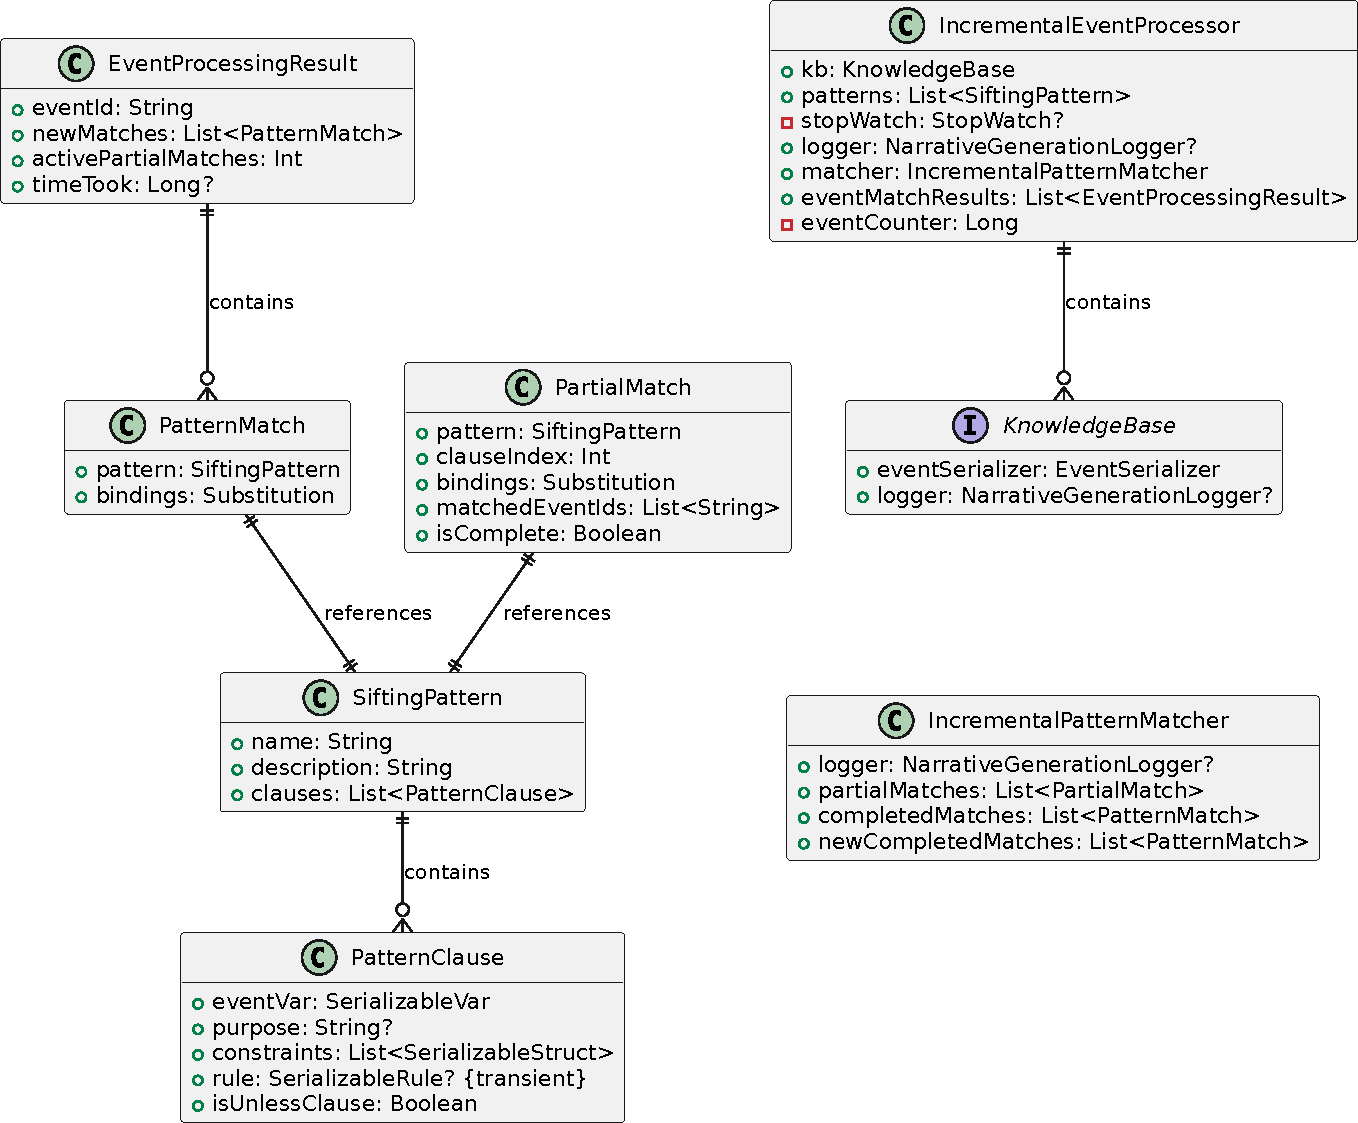
\includegraphics[width=\textwidth]{matchEngine.pdf}
    \caption{Class diagram of the main entities of the pattern-matching engine.}
    \label{fig:pattern-match-engine}
\end{figure}

The engine is designed to employ the incremental execution mode of Winnow.
%
This is achieved by maintaining a pool of partial matches.
%
Each time a new event is received, the engine attempts to match it against the first clause of all patterns to start new partial matches, and against the next expected clause of all active partial matches. If the event satisfies the condition of a clause, a new partial match is created.
%
Completed partial matches are removed from the pool.
%
In the original Winnow implementation, the previous partial match is left unchanged, so that it can be used to advance the match in other ways that might emerge later. 
%
This implementation instead consumes the prior partial match once it advances, so that only one path progresses per match instance.
%
Each complete match leads to exactly one log event, in order to avoid duplication and ambiguity in match reporting.
%
In both approaches, the new partial match inherits and extends the variable bindings based on the latest matching event.

As already stated in \cite{DBLP:conf/aiide/KreminskiDM21}, when managing a large collection of partial matches, the engine executes numerous small queries for each incoming event, at minimum one query per partial match.
%
These queries typically execute quickly despite their frequency. 
%
This efficiency stems from the fact that most logic variables have known values at query time, including the identifier of the event under evaluation and any variable bindings already captured in the partial match state.
%
This means that the query process only needs to verify a limited set of facts to determine potential bindings for the remaining unbound variables.

\subsection{Sifting pattern specification}

Winnow uses a custom external DSL inspired by Lisp to define patterns, as shown in \ref{listing:violation-of-hospitality-winnow}. 
%
This DSL is used to define Datalog queries over JSON data. 
%
It employs question marks to denote logical variables and the keywords \verb|pattern| and \verb|event| to denote the top level pattern and the building blocks that can compose them.
%
The \verb|where| keyword is used to declare the entries of each kind of block. The order with which the event blocks are defined enforce a constraint on the expected temporal ordering of events.

Since JaKtA is based on the 2p-kt \cite{DBLP:conf/woa/CiattoCSDO20} framework, it was decided to implement an internal DSL that employs Prolog in place of Datalog for defining the declarative rules for sifting.
%
This choice allows to benefit from the support of IDEs or text editors for Kotlin, providing various features that were not available with Winnow, like autocompletion, syntax highlighting, code navigation, folding and formatting, without incurring any additional maintenance burden.

\begin{listing}[ht]
\begin{minted}[fontsize=\small]{lisp}
(pattern violationOfHospitality
  (event ?e1 where
    eventType: enterTown,
    actor: ?guest)
  (event ?e2 where
    eventType: showHospitality,
    actor: ?host,
    target: ?guest,
    ?host.value: communalism)
  (event ?e3 where
    tag: harm,
    actor: ?host,
    target: ?guest))
\end{minted}
\caption{The violation of hospitality pattern as written in Winnow.}
\label{listing:violation-of-hospitality-winnow}
\end{listing}

\begin{listing}[ht]
\begin{minted}[fontsize=\small]{kotlin}
pattern("violationOfHospitality") {
    +event(E1) {
        +"type"(E1, "enterTown")
        +"agent"(E1, Guest)
    }

    +event(E2) {
        +"type"(E2, "showHospitality")
        +"agent"(E2, Host)
        +"target"(E2, Guest)
        +"value"(Host, "communalism")
    }

    +event(E3) {
        +"tag"(E3, "harm")
        +"type"(E3, HarmType)
        +"agent"(E3, Host)
        +"target"(E3, Guest)
    }
}
\end{minted}
\caption{The violation of hospitality pattern as written with the Kotlin DSL.}
\label{listing:violation-of-hospitality-kotlin}
\end{listing}

In \ref{listing:violation-of-hospitality-kotlin} an example of the Kotlin DSL is provided, which has the same semantics of the sifting pattern shown in \ref{listing:violation-of-hospitality-winnow}. The plus operator is used to denote event blocks. The keyword \verb|where| is no longer needed.

\section{Implementation Details}

The DSL allows to define how the description of the match is generated, both at the level of the single events and in how all the events are assembled to form a portion of the narration.
%
As shown in \ref{listing:out-of-stock-ordering} the \verb|meaning| extension function is used to define a formatted string that can be used to build the final event description.

\begin{listing}[!ht]
\begin{minted}[fontsize=\footnotesize]{kotlin}
pattern("OutOfStockOrdering") {
    +event(StockCheck) {
        +"type"(StockCheck, "BeliefAddition")
        +"belief_content"(StockCheck, "stock"(Thing, 0))
        +"agent"(StockCheck, Robot)
    }.meaning {
        +"$Robot detected $Thing is out of stock"
    }

    val msgPayload = "order"(Thing, Quantity).source("robot")

    +event(OrderEvent) {
        +"type"(OrderEvent, "SendMessage")
        +"message_from"(OrderEvent, Robot)
        +"message_type"(OrderEvent, "achieve")
        +"message_value"(OrderEvent, msgPayload)
        +"recipient"(OrderEvent, Supermarket)
    }.meaning {
        +"$Robot ordered more $Thing from $Supermarket"
    }

    description = """
        The ${eventClauses[0].purpose} so the ${eventClauses[1].purpose}
    """.trimIndent()
}
\end{minted}
\caption{Example sifting pattern for checking that when out of stock the robot orders new beer from the supermarket.}
\label{listing:out-of-stock-ordering}
\end{listing}

\begin{listing}
\begin{minted}[fontsize=\footnotesize]{prolog}
event_0_OutOfStockOrdering(Check, BeliefAddition, Thing, Robot) :-
    type(Check, BeliefAddition), 
    belief_content(Check, stock(Thing, 0)), 
    agent(Check, Robot).
event_1_OutOfStockOrdering(Order, SendMessage, Robot, Thing, Quantity, Supermarket) :-
    type(Order, SendMessage), 
    message_from(Order, Robot), 
    message_type(Order, achieve), 
    message_value(Order, order(source(robot), Thing, Quantity)), 
    recipient(Order, Supermarket).
\end{minted}
\caption{The prolog rules that are generated by the OutOfStockOrdering pattern.}
\label{listing:out-of-stock-ordering-prolog-rules}
\end{listing}

Each sifting pattern is converted to a set Prolog rules, one for each \verb|PatternClause|.
%
An example is provided in figure \ref{listing:out-of-stock-ordering-prolog-rules}.
%
Each log event is converted in a set of Prolog facts.
%
An example is provided in \ref{listing:prolog-event-conversion}.
%
The conversion of log events is performed by using reflection to get all the accessible properties of each \verb|LogEvent| and of its nested objects, up to a configurable maximum depth. A convention to name the functor is used, with an underscore for each level of the generated tree.
%
Since the name of the generated functors might become difficult to read or the extraction of data might become impractical, a system that allows to define custom mappings according to the type of the object has been devised. 
%
This allows to override the functor naming convention or to ignore certain properties of an object when needed.
%
An an example, the system is used in \ref{listing:prolog-event-conversion} to allow easier access to the belief source and content, by generating derived facts from \verb|belief_rule|.

\begin{listing}
\begin{minted}[fontsize=\footnotesize]{prolog}
belief_source(event_21, 'Self').
belief_content(event_21, too_much(Thing1)).
belief_rule(event_21, too_much(source(self), Thing1)).
change_type(event_21, 'ADDITION').
description(event_21, 'Added too_much(Thing_2) from source Self').
type(event_21, 'BeliefAddition').
time(event_21, 1748874972229).
agent(event_21, robot).
\end{minted}
\caption{The prolog rules that are generated for a BeliefAddition log event.}
\label{listing:prolog-event-conversion}
\end{listing}

The project initially used Slf4j with Logback for logging, but this combination presented several limitations. 
%
Most notably, it lacked support for using custom serialization libraries and for logging custom JSON objects.
%
This meant that objects could only be logged using escaped characters by providing raw JSON strings, by defining custom Jackson serializers or by providing custom key-values at the top level or in the MDC context.
%       
The migration to Log4j addressed these limitations. Log4j allows direct object logging and, with the newer and more performant \verb|JsonTemplateLayout|, enables the integration with any serialization library.
%
This allowed to reuse the kotlinx serialization library, which is already used in other parts of the project and provides better integration with the Kotlin codebase.
%
The architectural advantages of Log4j also influenced this decision. Since Log4j maintains a clear separation between its API and core components, there was no real reason to continue using Slf4j as an abstraction layer. 
%
Additionally, Log4j offers a superior API for building loggers programmatically compared to Logback.

To optimize performance, lambdas have been employed to avoid costly computations during logging operations. This approach is roughly similar to the strategy used in the \href{https://github.com/oshai/kotlin-logging}{kotlin-logging} library, but has been specifically adapted to work with Log4j's API. This implementation is effective because it leverages the underlying Log4j API that uses Java suppliers, which supports the conditional evaluation of log messages and parameters according to the currently enabled log level.

\section{Evaluation}
\subsection{Requirements Validation}

The requirements have been addressed since:

\begin{itemize}
    \item the project allows to store the execution traces of a mas;
    \item declarative Prolog rules to match patterns can be built using an internal DSL;
    \item the pattern matching engine and the pattern builder implementations are clearly separated;
    \item by reusing the technique implemented in Winnow, incremental matching is supported and it can be used to handle a stream of log events.
\end{itemize}

The non functional-requirements have been addressed since:

\begin{itemize} 
    \item Extensibility: new log events can be defined by extending the \verb|LogEvent| interface, while new patterns can be defined using the DSL. A \href{https://github.com/pikalab-unibo-students/master-thesis-battistini-ay2425/blob/feat/jakta-sifting-patterns/jakta-playground/src/main/kotlin/it/unibo/jakta/playground/evaluation/scripts/EventReferenceGenerator.kt}{script} can be run to create a reference file that shows what kind of rules can be written to extract data from each event.
    \item Compatibility: the integration with existing JaKtA applications is straighforward since the only requirement for logging and pattern-matching is adding a \verb|LoggingConfig| instance in the \verb|mas| block of the JaKtA DSL.
\end{itemize}

The implicit requirements have been partially addressed since:

\begin{itemize}
    \item Performance: if five patterns are used, matching an event requires on average six milliseconds, so two thousand and five hundred events require about fifteen seconds. In the limited context of the toy example analyzed, the requirement can be considered satisfied. The logging system is well optimized and the \href{https://logging.apache.org/log4j/2.x/manual/performance.html}{best practices}  have been followed.
    \item Scalability: concurrency is only partially addressed. Timestamps with nanosecond resolution can be used to process the log events generated by agents running concurrently on a single node  while keeping the temporal ordering of the events. For the online processing, if each agent runs in its separate thread then there is no guarantee that the events are ordered. In such a case a more advanced matching engine would be needed, that for example keeps a buffer with events ordered by timestamp.
    \item Structure: using a serialization library and extending Log4j2 with custom plugins, both the raw execution traces and the ones obtained from pattern matching can be stored in JSON Lines files.
\end{itemize}

\subsection{Domestic Robot application}

The system is evaluated using the Domestic Robot domain, where the robot agent manages beer-serving requests, stock monitoring, and automated ordering. The domain is described below.

\begin{displayquote}
A domestic robot has the goal of serving beer to its owner. Its mission is
quite simple, it just receives some beer requests from the owner, goes to the
fridge, takes out a bottle of beer, and brings it back to the owner.
However, the robot should also be concerned with the beer stock (and eventually
order more beer using the supermarket’s home delivery service) and some rules
hard-wired into the robot by the Department of Health (in this example this
rule defines the limit of daily beer consumption).
\end{displayquote}

From the analysis of the domain, the following set of main features to validate has been defined:

\begin{itemize}
    \item Beer Request and Delivery: the robot fetches and delivers beer to owner on demand when stock is available and daily limits aren't exceeded.
    \item Daily Limit Enforcement: the robot refuses beer requests when owner has reached their daily consumption limit per health regulations.
    \item Out of Stock Handling: the robot automatically orders more beer from the supermarket when owner requests beer but none is available.
    \item Beer Delivery from Supermarket: the supermarket processes robot's beer orders and delivers stock to replenish inventory.
    \item Owner's Time Check Behavior: the robot provides the current time information when the owner asks it.
\end{itemize}

A set of sifting patterns was implemented to verify each of these features. They are available in the \verb|it.unibo.jakta.playground.domesticrobot.patterns| package. As an example the ones for the Beer Request and Delivery and the Beer Delivery from Supermarket are shown in listings \ref{listing:beer-request-delivery-pattern} and \ref{listing:beer-delivery-supermarket-pattern}. In listings \ref{listing:beer-request-delivery-feature} and \ref{listing:beer-delivery-supermarket-feature} the description of the associated feature for each of them is reported.

\begin{listing}
\begin{minted}[fontsize=\small]{kotlin}
pattern("ThingRequestAndDelivery") {
    +event(RequestEvent) {
        +"type"(RequestEvent, "MessageReceived")
        +"message_from"(RequestEvent, Owner)
        +"message_type"(RequestEvent, "achieve")
        +"message_value"(RequestEvent, "has"(Owner, Thing))
        +"agent"(RequestEvent, Robot)
    }.meaning {
        +"$Owner requested $Thing from $Robot"
    }
    +event(FetchEvent) {
        +"type"(FetchEvent, "ActionSuccess")
        +"action_signature_name"(FetchEvent, "pick")
        +"provided_arguments"(FetchEvent, Thing)
        +"agent"(FetchEvent, Robot)
    }.meaning {
        +"$Robot took $Thing from the fridge"
    }
    +event(DeliverEvent) {
        +"type"(DeliverEvent, "BeliefAddition")
        +"belief_content"(DeliverEvent, "has"(Owner, Thing))
        +"agent"(DeliverEvent, Owner)
    }.meaning {
        +"$Robot delivered $Thing to $Owner"
    }
}
\end{minted}
\caption{The ThingRequestAndDelivery pattern, which is used to verify that the Beer Request and Delivery feature correctly works.}
\label{listing:beer-request-delivery-pattern}
\end{listing}

\begin{listing}
\begin{minted}[fontsize=\small]{text}
Feature: Beer Request and Delivery

As an owner,
I want to request beer from my robot,
so that I can receive it without leaving my seat.

Scenario: Beer delivered when available

Given the owner requests a beer,
When there is beer in stock and daily limit not reached,
Then the robot fetches beer from the fridge and delivers it to the owner.
\end{minted}
\caption{The Beer Request and Delivery feature from which the pattern ThingRequestAndDelivery was created.}
\label{listing:beer-request-delivery-feature}
\end{listing}

\begin{listing}
\begin{minted}[fontsize=\small]{kotlin}
pattern("ThingDelivery") {
    val msgPayload = "order"(Thing, Quantity).source("robot")
    +event(OrderReceived) {
        +"type"(OrderReceived, "MessageReceived")
        +"message_from"(OrderReceived, Robot)
        +"message_type"(OrderReceived, "achieve")
        +"message_value"(OrderReceived, msgPayload)
        +"agent"(OrderReceived, Supermarket)
    }.meaning {
        +"$Supermarket received order for $Quantity ${Thing}s from $Robot"
    }
    +event(DeliveryEvent) {
        +"type"(DeliveryEvent, "SendMessage")
        +"message_from"(DeliveryEvent, Supermarket)
        +"message_type"(DeliveryEvent, "tell")
        +"message_value"(DeliveryEvent, "delivered"(Thing, Quantity, OrderId))
        +"recipient"(DeliveryEvent, Robot)
    }.meaning {
        +"$Supermarket delivered $Quantity ${Thing}s to $Robot"
    }
}
\end{minted}
\caption{The ThingDelivery pattern, which is used to verify that the Beer Delivery from Supermarket feature correctly works.}
\label{listing:beer-delivery-supermarket-pattern}
\end{listing}

\begin{listing}
\begin{minted}[fontsize=\small]{text}
Feature: Beer Delivery from Supermarket

As a supermarket,
I want to process and deliver beer orders from robots,
so that they can maintain their stock.

Scenario: Order processed and delivered

Given the robot has ordered beer from the supermarket,
When the supermarket processes the order,
Then the supermarket delivers the beer to the robot and updates its beer stock.
\end{minted}
\caption{The Beer Delivery from Supermarket feature from which the pattern ThingDelivery was created.}
\label{listing:beer-delivery-supermarket-feature}
\end{listing}

An example of the narrative generated by the application is shown in \ref{listing:example-narrative}.

\begin{landscape}
\begin{listing}
\begin{minted}[fontsize=\scriptsize]{text}
The owner asked robot for the time so the robot told owner that the current time is: '2025-06-02 14:36:13.661075'
...
The owner asked robot for the time so the robot told owner that the current time is: '2025-06-02 14:36:21.624622'
The owner requested beer from robot, so the robot took beer from the fridge and robot delivered beer to owner 
The owner asked robot for the time so the robot told owner that the current time is: '2025-06-02 14:36:25.215372'
The owner asked robot for the time so the robot told owner that the current time is: '2025-06-02 14:36:27.020011'
The robot detected beer is out of stock so the robot ordered more beer from supermarket
Since the supermarket received order for 3 beers from robot the supermarket delivered 3 beers to robot
The owner asked robot for the time so the robot told owner that the current time is: '2025-06-02 14:36:29.465186'
...
The owner asked robot for the time so the robot told owner that the current time is: '2025-06-02 14:36:36.171572'
The owner requested beer from robot, so the robot took beer from the fridge and robot delivered beer to owner 
The owner asked robot for the time so the robot told owner that the current time is: '2025-06-02 14:36:38.871042'
...
The owner asked robot for the time so the robot told owner that the current time is: '2025-06-02 14:36:48.789099'
The owner requested beer from robot, so the robot took beer from the fridge and robot delivered beer to owner 
The owner asked robot for the time so the robot told owner that the current time is: '2025-06-02 14:36:51.599050'
...
The owner asked robot for the time so the robot told owner that the current time is: '2025-06-02 14:37:04.676487'
The owner requested beer from robot, so the robot took beer from the fridge and robot delivered beer to owner 
The owner asked robot for the time so the robot told owner that the current time is: '2025-06-02 14:37:08.046887'
The owner asked robot for the time so the robot told owner that the current time is: '2025-06-02 14:37:10.043639'
The robot detected beer is out of stock so the robot ordered more beer from supermarket
Since the supermarket received order for 3 beers from robot the supermarket delivered 3 beers to robot
The owner asked robot for the time so the robot told owner that the current time is: '2025-06-02 14:37:12.853566'
...
The owner asked robot for the time so the robot told owner that the current time is: '2025-06-02 14:37:19.671028'
The owner requested beer from robot, so the robot took beer from the fridge and robot delivered beer to owner 
The owner asked robot for the time so the robot told owner that the current time is: '2025-06-02 14:37:22.254820'
The owner asked robot for the time so the robot told owner that the current time is: '2025-06-02 14:37:25.813696'
Since the owner requested beer from robot and the daily limit has been reached, the robot informed owner about reaching daily limit.
\end{minted}
\caption{The domain-level log events extracted from the execution trace of the Domestic Robot application. For brevity ellipsis are used to omit additional occurrences of the robot reporting the time to the owner.}
\label{listing:example-narrative}
\end{listing}
\end{landscape}

\subsection{Test suite}

The custom serializers provided for the log events have been tested with a subset of the log events of the BDI engine. They are available in the \\ \verb|it.unibo.jakta.agents.bdi.engine.serialization| package.

The incremental pattern matching engine correctedness is verified with a test provided under the \verb|it.unibo.jakta.agents.bdi.narrativegenerator| package.

\section{Deployment Instructions}

The deployment for the offline scenario requires issuing the following commands:

\begin{minted}[fontsize=\footnotesize]{bash}
git clone https://github.com/pikalab-unibo-students/master-thesis-battistini-ay2425
git checkout feat/jakta-sifting-patterns
cd master-thesis-battistini-ay2425
\end{minted}

The online scenario uses a centralized logging system, based on the \href{https://www.elastic.co/elastic-stack/}{ELK stack} (with Opensearch in place of Elastic).
%
To deploy the single-node cluster in development mode a docker compose file can be used:

\begin{minted}[fontsize=\footnotesize]{bash}
cd jakta-toolbox/infra
docker compose up
\end{minted}

Both the \href{https://docs.docker.com/engine/install/}{Docker Engine} and \href{https://docs.docker.com/compose/install/}{Docker Compose} need to be installed.
%
The compose file will build an extended version of Logstash with the plugin to work with OpenSearch. 
%
In addition, it will read the configuration of the instance from the \verb|logstash.conf| file on the filesystem, it will bind ports 9200 and 4054-4056 and create a volume to store the server data.

\section{Usage Examples}

Since the matching of the sifting patterns can be performed both online and offline, an example is given below for each of the two scenarios.

\subsection{Online scenario}

To perform pattern matching in an online manner, make sure to deploy the ELK cluster as outlined before, then start the Ktor application that will perform the enrichment of the logs.
%
Finally, once the server is ready, the domestic robot application can be started.

\begin{minted}[fontsize=\footnotesize]{bash}
./gradlew matchStream
./gradlew runDomesticRobot --args="--log-to-server --log-to-file --log-to-single-file"
\end{minted}

This will produce a set of logs that will be stored in the OpenSearch instance and printed on console by the \verb|matchStream| task.
%
To print the stored logs on stdout, the following Gradle task can be run:

\begin{minted}[fontsize=\footnotesize]{bash}
./gradlew analyzeIndex --args="--mas-id <id> --implementation-level"
\end{minted}

Where the \verb|--mas-id| option requires the UUID generated by the execution of the \verb|runDomesticRobotSample| task and available by reading the file name of the log file written under the \verb|jakta-playground/logs| directory.

To see the logs generated by the pattern-matching, the following task can be used:

\begin{minted}[fontsize=\footnotesize]{bash}
./gradlew analyzeIndex --args="--mas-id <id> --domain-level"
\end{minted}

\subsection{Offline scenario}

Pattern matching in the offline manner requires running the following Gradle tasks:

\begin{minted}[fontsize=\footnotesize]{bash}
./gradlew runDomesticRobot --args="--log-to-file --log-to-single-file"
./gradlew matchFile --args="--log-to-file --match-file '$PWD/jakta-playground/logs/trace-<id>.jsonl'"
\end{minted}

The first task will write the log file with the execution trace of the system on the local filesystem and print it on the console.
%
The second task requires specifying the path to the generated log file, which includes a UUID printed to console by the previous task. The result will be the new log events generated by the pattern matching.
%
Both tasks will write to the \verb|jakta-playground/logs| directory.

\section{Conclusions}

In its current state, the project allows to define declarative rules, in the form of sifting patterns in a Kotlin DSL, to generate a set of new log events that explain the behavior of one or more agents at a higher level of abstraction than what the raw logs afford.

\subsection{Future Works}

The reference work by Yan et al. \cite{DBLP:journals/aamas/YanBHR25} does define a set of mappings that have not been fully implemented in this project.
%
In particular, the implementation level contains many events that should belong to the design level according to the original theorization.
%
A first step would then be to redefine the set of events that get logged at the implementation level, both to reduce the current amount of generated log traces and to properly define the design level with a set of sifting patterns that use the implemented DSL.

The project currently implements a subset of the features provided by Winnow.
%
The most notable missing one is the unless-event clause, which can be used to invalidate partial matches if a certain event with a certain set of constraints happens between other events of the pattern. 
%
Currently, all the events that do not match an event block are ignored and partial matches are removed only when a pattern is completely matched.

To provide support for structured logging, a set of custom kotlinx serializers have been implemented, in order to integrate with the 2p-kt classes. 
%
All the classes extending the \verb|LogEvent| interface where made serializable.
%
That said, 2p-kt already provides modules for serialization that use Jackson and the current kotlinx serialization does not handle all subtypes of the \verb|Term| class.
%
So a future development might be either to reuse the serializers provided by the framework or fully reimplement them with custom kotlinx serializers.

The current logging implementation is tightly coupled with the BDI engine. 
%
An event-driven architecture can be implemented, by leveraging Kotlin Flows, to define a separate logging module that registers as a listener for log events.
%
This approach might also be used to implement testing frameworks, as the one in \cite{DBLP:conf/ecai/PiresS24}, to listen for engine events and validate the behavior of BDI agents.
%
Test assertions can be made based on the sequence and content of the emitted events, enabling the validation of the agents' behavior without modifying the BDI engine.

Other interesting future developments might revolve around the use of the high-level narratives generated with the system:

\begin{itemize}
\item to provide more context to an LLM that augments the deliberation cycle of an agent, for example for performing plan selection or plan generation;
\item for plan or goal recognition, so that both BDI and LLM agents might try to infer the behavior of other agents according to a set of handcrafted or procedurally-generated sifting patterns.
\end{itemize}

\subsection{What did I learn}

This project significantly improved my understanding of the BDI agent architecture through hands-on exploration of the JaKtA BDI interpreter's internal mechanisms. 

I also had the opportunity to experiment with cutting-edge research in autonomous agents by implementing a system based on existing work on explainability and integrating it with approaches coming from complementary AI research domains.

\nocite{*}
\bibliographystyle{plain}
\bibliography{references}

\end{document}